% !TEX root = ../../sethomas_thesis_main.tex
\documentclass[border=1mm,
               class=article
               preview]{standalone}
\usepackage{tikz}
\begin{document}
\begin{tikzpicture}
    \node[anchor=south west,inner sep=0] (graph) at (0,0) {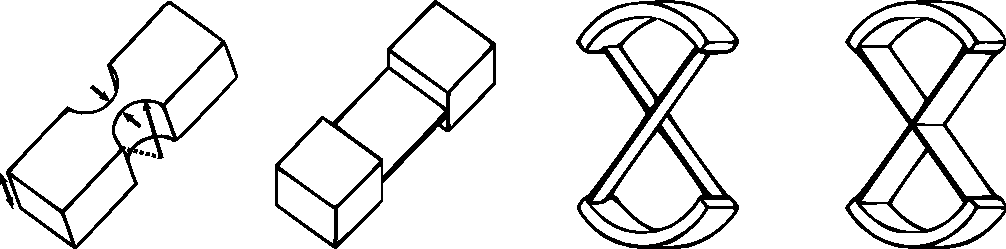
\includegraphics[width=\textwidth]{images/chap4/flexure-hinge-types-arrows.pdf}};
    \begin{scope}[x={(graph.south east)},y={(graph.north west)}]
        \node at (0.065,-0.15) {\textbf{(a)}};
        \node at (0.33,-0.15) {\textbf{(b)}};
        \node at (0.65,-0.15) {\textbf{(c)}};
        \node at (0.92,-0.15) {\textbf{(d)}};

        \node at (-0.01,0.21) {$b$};
        \node at (0.08,0.645) {$e$};
        \node at (0.175,0.385) {$r$};
    \end{scope}
    \end{tikzpicture}%
\end{document}
